\documentclass[12pt]{article}

\title{Natural caustics in backward path tracing}
\author{
Shawn Halayka\footnote{sjhalayka@gmail.com}
}


\date{\today\;\currenttime}

\usepackage{datetime}
\usepackage{listings}
\usepackage{cite}
\usepackage{xcolor}
\usepackage{graphicx}
\usepackage{setspace}
\usepackage{amsmath}
\usepackage{url}
\usepackage{amsfonts}
\usepackage{caption}
\usepackage{subcaption}

\usepackage[margin=1in]{geometry}

%\doublespace

\begin{document}

\newcommand{\abs}[1]{\lvert#1\rvert}



\maketitle




\begin{abstract}
In this paper we introduce a natural method for producing both refraction and reflection caustics in backward path tracing (e.g. bouncing around an eye ray in the scene until a light is found).
These caustics do not rely on a light location, and as such, do not rely on bidirectional or forward path tracing.
As such, these caustics allow for as many light sources as one would care for; the shapes and positions of the lights are completely arbitrary (can be bunny shaped, etc).
We use the standard Cornell box for testing the backward path tracer.
\end{abstract}







\section{Rasterizer versus ray tracer versus backward path tracer}

The three main visualization algorithms in contemporary graphics programming are the rasterizer \cite{noll, wikipedia1}, ray tracing \cite{appel, wikipedia2}, and path tracing \cite{kajiya, wikipedia3}.

The rasterizer literally converts vector graphics (generally: triangles, lines, and points, all collectively known as simplices) into raster graphics (pixels, also known as fragments).
Generally, a depth buffer (Z-buffer) \cite{wikipedia4} is used to discern which fragments for each simplex to draw, or which to discard, depending on distance to the eye and also what fragments that have been previously drawn.
This depth testing algorithm is super simple, and it does the job, but it is just simply not as programmable as a ray tracer or backward path tracer.
See Fig. 1 for an example render performed by the rasterizer.

The ray tracer does a similar job, insomuch that it converts triangles into pixels.
Rather than using a depth buffer though, one often uses a more complicated acceleration structure, such a bounding volume hierarchy (BVH) \cite{wikipedia5}, to determine eye ray / triangle intersection.
See Fig. 2 for an example render performed by ray tracing.

The backward path tracer is identical to the ray tracer, except that it also takes global illumination into account.
The backward path tracer often uses the exact same acceleration structure setup as the ray tracer.
It's worth noting that the construction of the acceleration structure is handled for you by the Vulkan / Direct3D 12 driver, which adds to the naturalness of the caustics discussed in this paper.

Here we rate the three main visualization algorithms.
We rate them in terms of what is relatively easy, or naturally occurring, in each of the visualization algorithms.
\begin{center}
\begin{tabular}{| l | r | r | r | r |}
  \hline
 Algorithm &  Reflections & Shadows & Refraction caustics & Reflection caustics \\
\hline
\hline
Rasterizer & No & No & No &  No \\
Ray tracer & Yes & Sharp & No & No  \\
Backward path tracer & Yes & Sharp / soft & Yes & Yes \\
  \hline  
\end{tabular}
\end{center}
Clearly, the most suitable visualization algorithm for now (and in the future) is the backward path tracer.
This is not to say that, for instance in the case of the rasterizer, there is no such thing as shadows.
It's just that the implementation of shadows is a kludgy affair, or not naturally occurring.

Although caustics can be produced using bidirectional or forward path tracing, they suffer from convergence (or lack thereof) problems.
These particular issues do not plague the backward path tracer.






\section{The old special backward path tracing algorithm}

Each eye ray is sent out $s$ times, each referred to as a sample.

Essentially, each eye ray sample is bounced around pseudorandomly as it hits surfaces within the scene.
The bounce count is finite, and bouncing stops after $n$ bounces, or if a light is hit, or if the sky is hit.
At each bounce, one takes into account the properties of the surface, such as colour.

In the end, the eye ray's final colour is divided by the sample count.

This works great for diffuse, opaque surfaces.

If there is a so-called convergence problem with regard to the backward path tracer's output, it's because there are not enough samples being taken.
Samples take time, but they produce beautiful results.

See Fig. 3 for the old code, in GLSL.





\section{The new general backward path tracing algorithm}

Other than diffuse, opaque surfaces, there are reflective and transparent surfaces to consider.
One can generalize the old algorithm by adding in code to handle reflective and transparent surfaces.

Everything is the same as the old special backward path tracer, except that now each bounce accounts for the extended properties such as reflectivity and transparency.
That is, rather than always pseudorandomly bouncing the eye ray around, one will also be able to reflect the eye ray if the surface is reflective, and one will refract the eye ray if the surface is transparent.

See Fig. 4 for the new code, in GLSL.

See Figs. 5 - 10 for the results of the new code.
Each image is rendered at a size of 7680 x 4204, at $s = 25$ samples per eye ray with maximum $n = 5$ bounces, then cropped and downsized to like 1000 x 1000.
The full size images are available upon request.






\section{Photon mapping versus the backward path tracer}

Comparing this backward path tracer to photon mapping \cite{jensen, john} is like comparing apples and oranges.

For one, photon mapping uses a kd tree for storing photon data, and the backward path tracer does not.
It takes time and space to store and retrieve data to and from the photon map.

For another, path tracing has a future -- this is to say that, on an NVIDIA 3060 laptop GPU, the backward path tracer is still at best only an offline renderer at 4K resolution.
Its day will come.

Finally, it must be noted that the backward path tracer is strictly a view space effect.
This is unlike photon mapping and its 2-pass solution, insomuch that the caustics and other lighting effects are all accomplished in one pass when using the backward path tracer.

It should be noted that photon mapping also suffers from its own inherent convergence problems (e.g. low photon count).
These particular issues do not plague the backward path tracer.

In essence, photon mapping is a kludge when compared to the ease and naturalness of the caustics in the backward path tracer.





\section{Acknowledgements}

The code for this paper is based off of Sascha Willems' and NVIDIA's work \cite{willems1, willems2, nvidia}.

The various Cornell boxes were developed by Rob Rau.

The code and various Cornell boxes can be found at: 

\url{https://github.com/sjhalayka/cornell_box_textured}



\pagebreak




\begin{thebibliography}{9}

\bibitem{noll} Noll. Scanned-display computer graphics.
\bibitem{wikipedia1} Wikipedia. Rasterisation.

\bibitem{appel} Appel. Some techniques for shading machine renderings of solids.
\bibitem{wikipedia2} Wikipedia. Ray tracing.

\bibitem{kajiya} Kajiya. The rendering equation.
\bibitem{wikipedia3} Wikipedia. Path tracing.

\bibitem{wikipedia4} Wikipedia. Depth buffering (Z-buffering).
\bibitem{wikipedia5} Wikipedia. Bounding volume hierarchy.


\bibitem{jensen} Jensen. Realistic image synthesis using photon mapping.
\bibitem{john} John. Focus on photon mapping.

\bibitem{willems1} Willems. Vulkan path tracer.
\bibitem{willems2} Willems. Vulkan examples and demos.
\bibitem{nvidia} NVIDIA. Vulkan mini path tracer.



\end{thebibliography}


\pagebreak







\begin{figure} 
\centering
  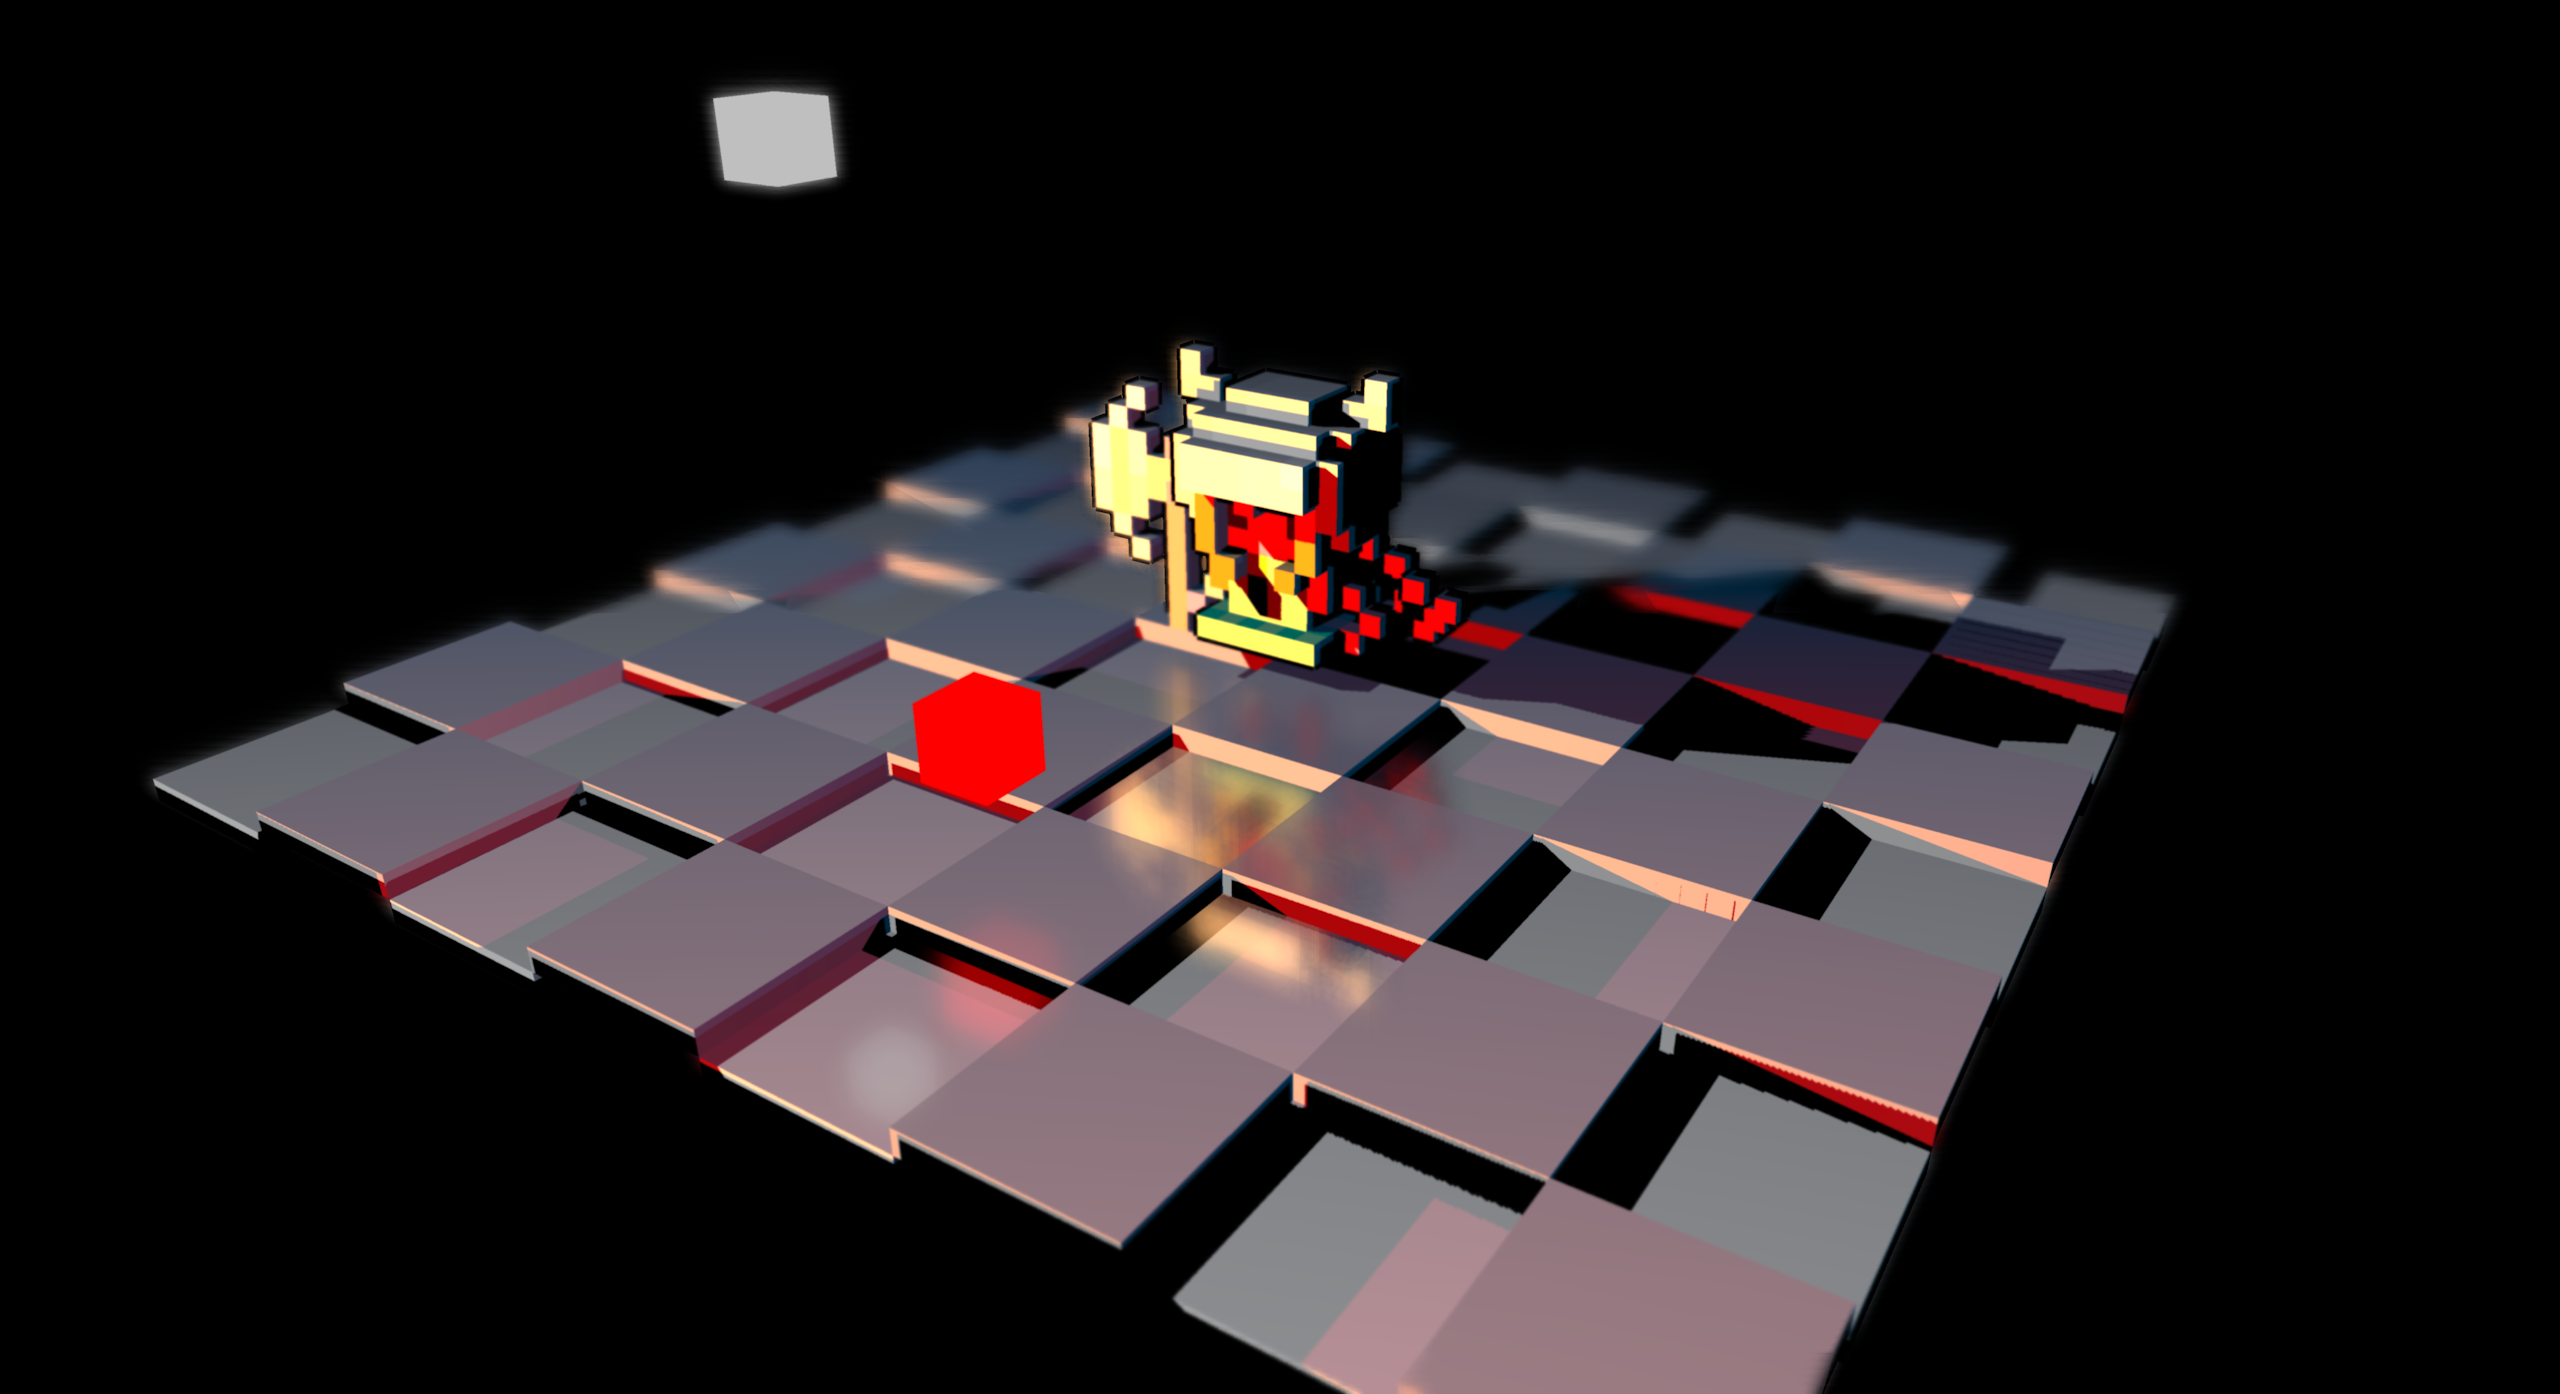
\includegraphics[width = 6 in]{fig1.png}
  \caption{ Rasterizer.
The surface is lit using Phong shading and omnidirectional shadow maps.
The reflections are faked -- the camera is flipped upside down, and reflected things masked and drawn.
In other words, reflections and shadows are not naturally occurring.
Global illumination is not taken into account.
This knight model was made by the Twitter user @ephtracy.
}

\end{figure}






\begin{figure} 
\centering
  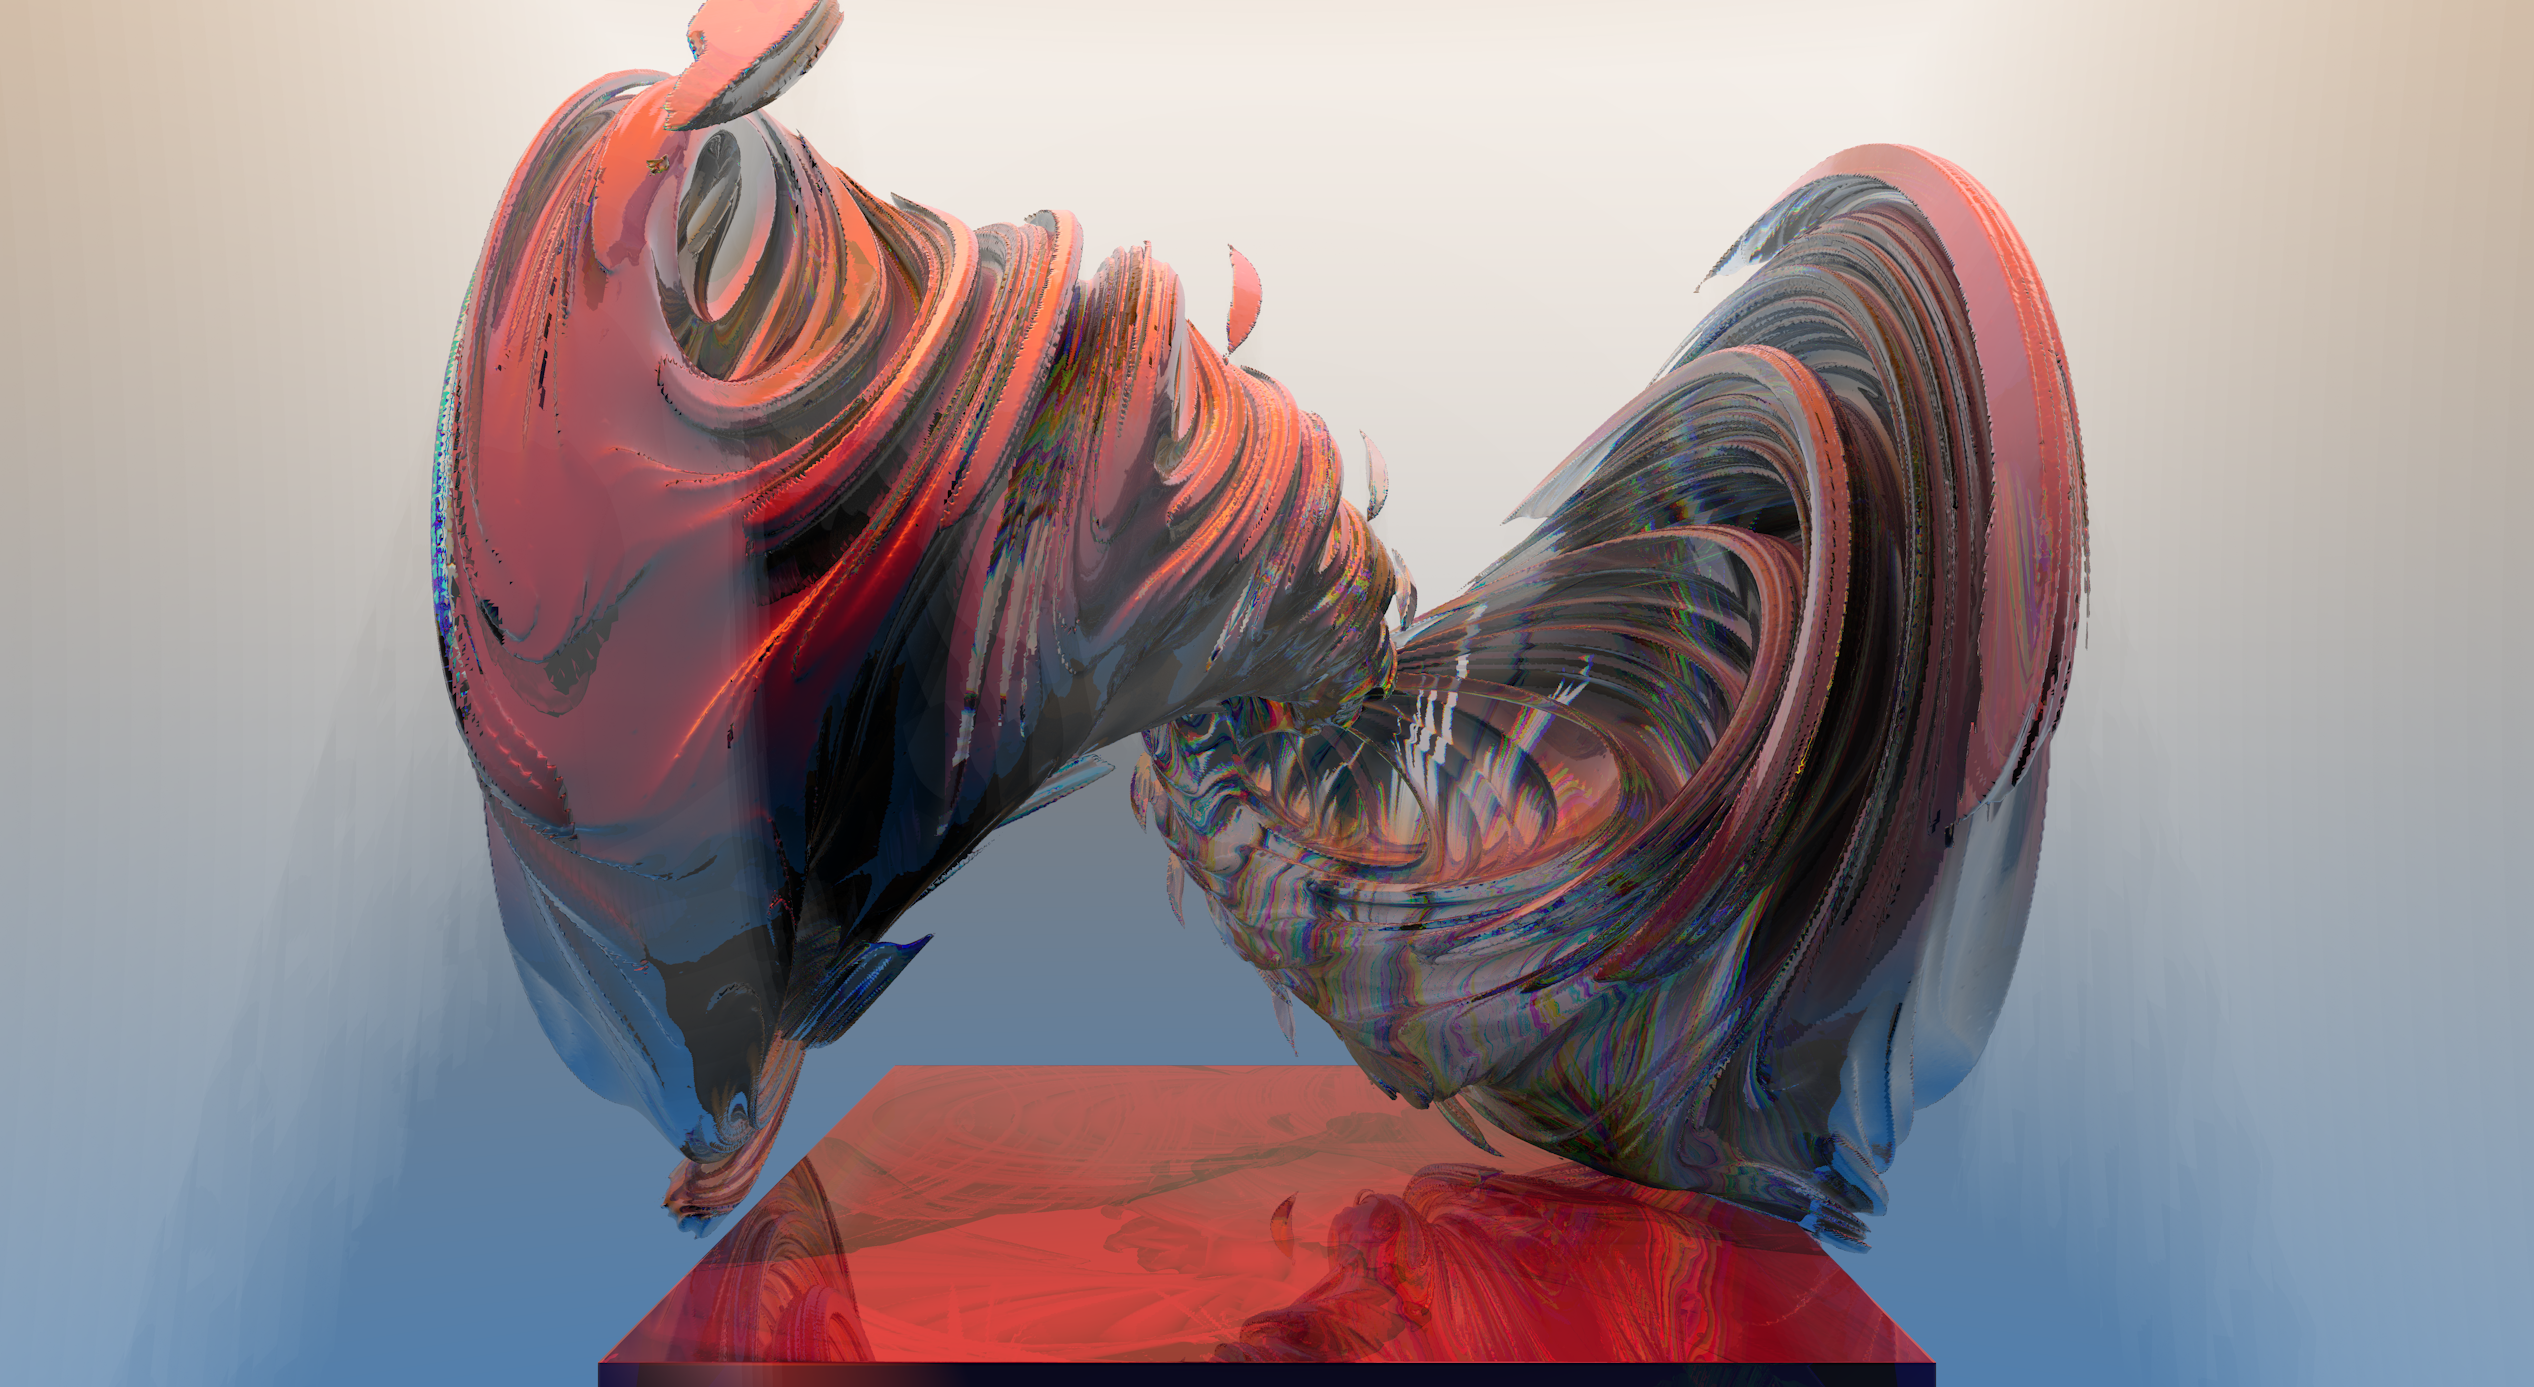
\includegraphics[width = 6 in]{fig2.png}
  \caption{ Ray tracer, taking into account transparency.
The surface is lit using Phong shading and sharp shadows.
In other words, reflections and shadows are naturally occurring.
Global illumination is not taken into account.
}
\end{figure}




\begin{figure} 
\centering
  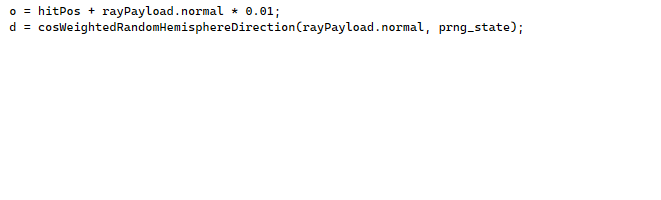
\includegraphics[width = 6 in]{fig3.png}
  \caption{ Old backward path tracer code, always using a pseudorandom cosine-weighted direction vector (e.g. scattering).
Here the o variable is the ray origin, and d is the ray direction.
Works great for opaque diffuse surfaces.
}
\end{figure}






\begin{figure} 
\centering
  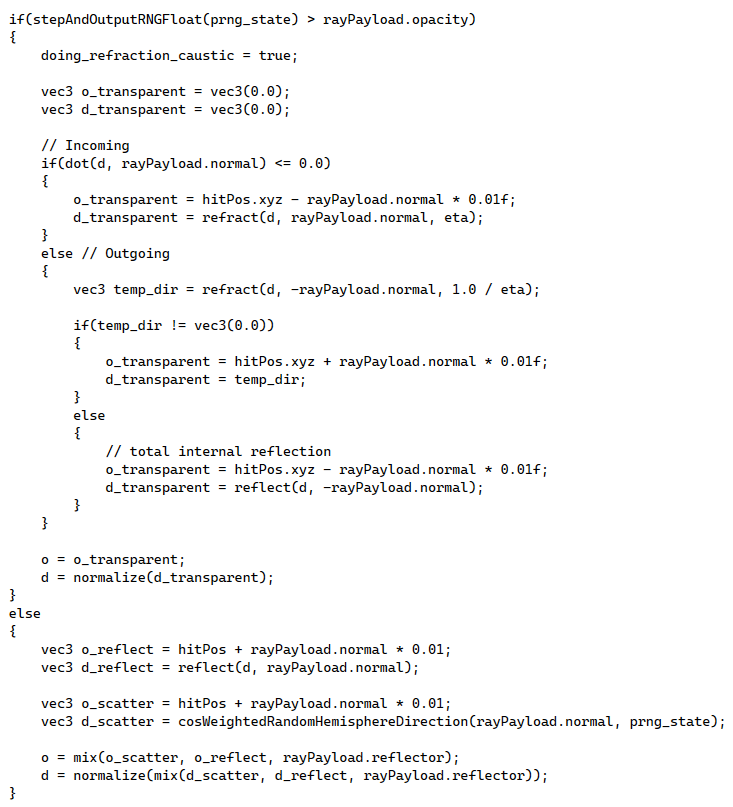
\includegraphics[width = 6 in]{fig4.png}
  \caption{ New backward path tracer code, taking reflective and transparent surfaces into consideration.
This solution for caustics performs well on modern graphics provessing units -- disabling caustics causes a practically imperceptible gain in frame rate.
While not as simple as the old backward path tracer code, it is still not very computationally expensive -- just the right amount of complexity leads to much better results.
}
\end{figure}

\begin{figure} 
\centering
  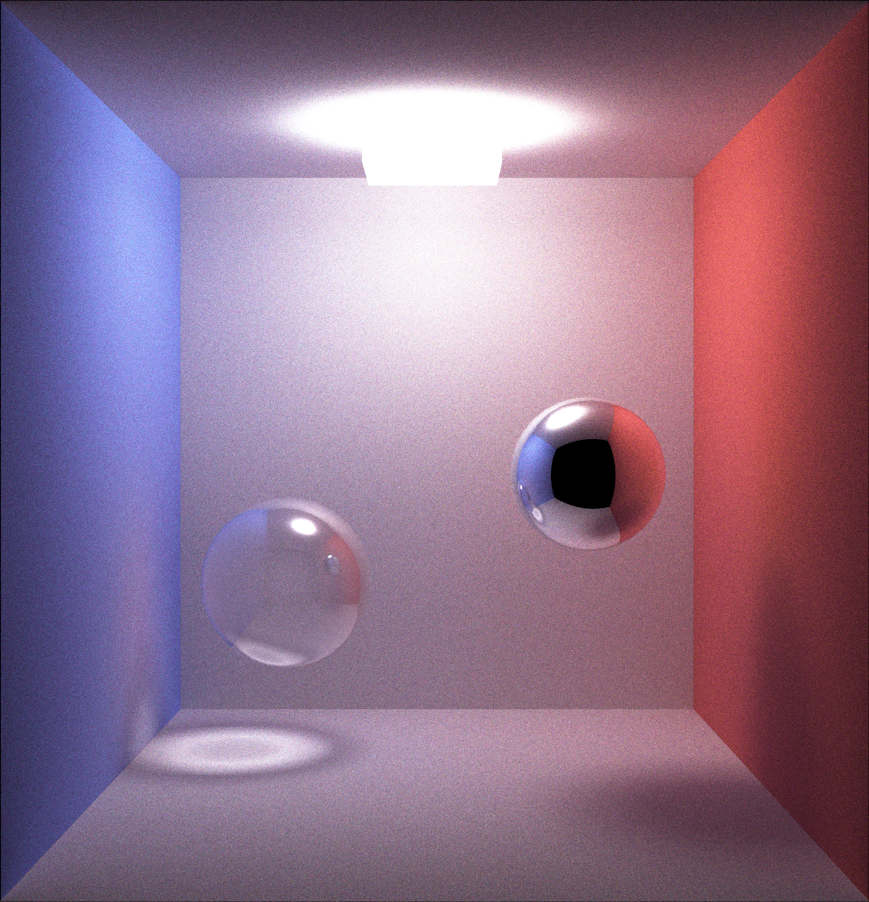
\includegraphics[width = 6 in]{fig5.png}
  \caption{  Backward path tracer, taking transparent surfaces into consideration. 
Note the naturally occurring refraction caustic.
Note the soft shadows.
Global illumination (e.g. colour bleeding / indirect lighting) is taken into account.
}
\end{figure}


\begin{figure} 
\centering
  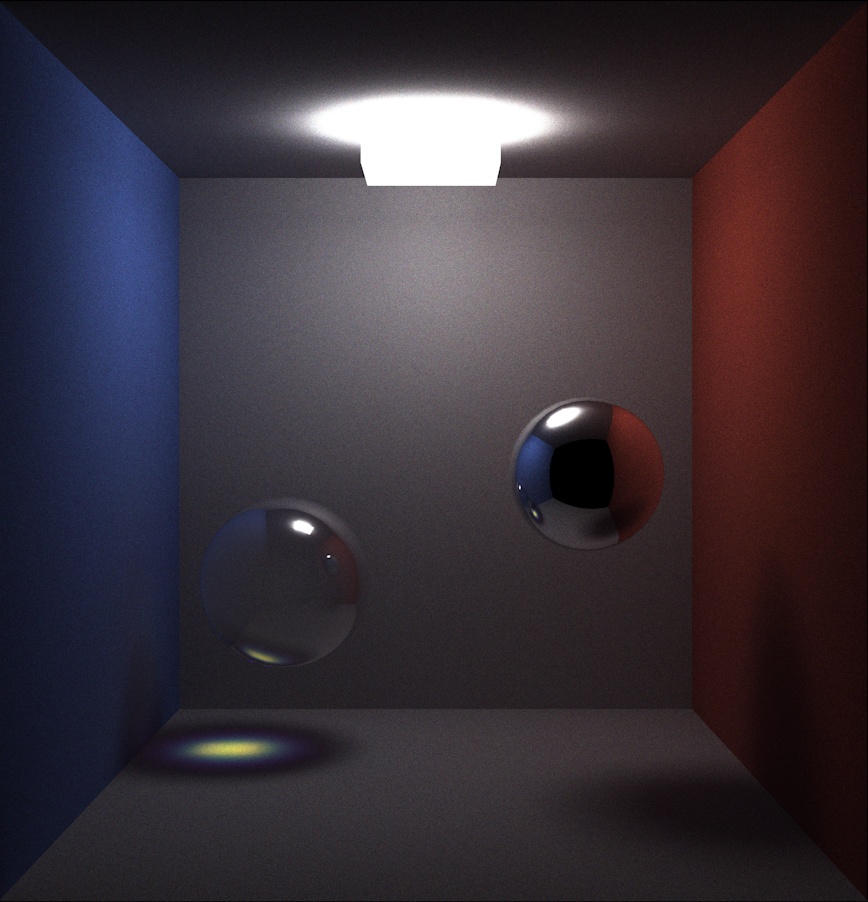
\includegraphics[width = 6 in]{fig6.png}
  \caption{ Note the refraction caustic, with 20-channel chromatic aberration.
}
\end{figure}

\begin{figure} 
\centering
  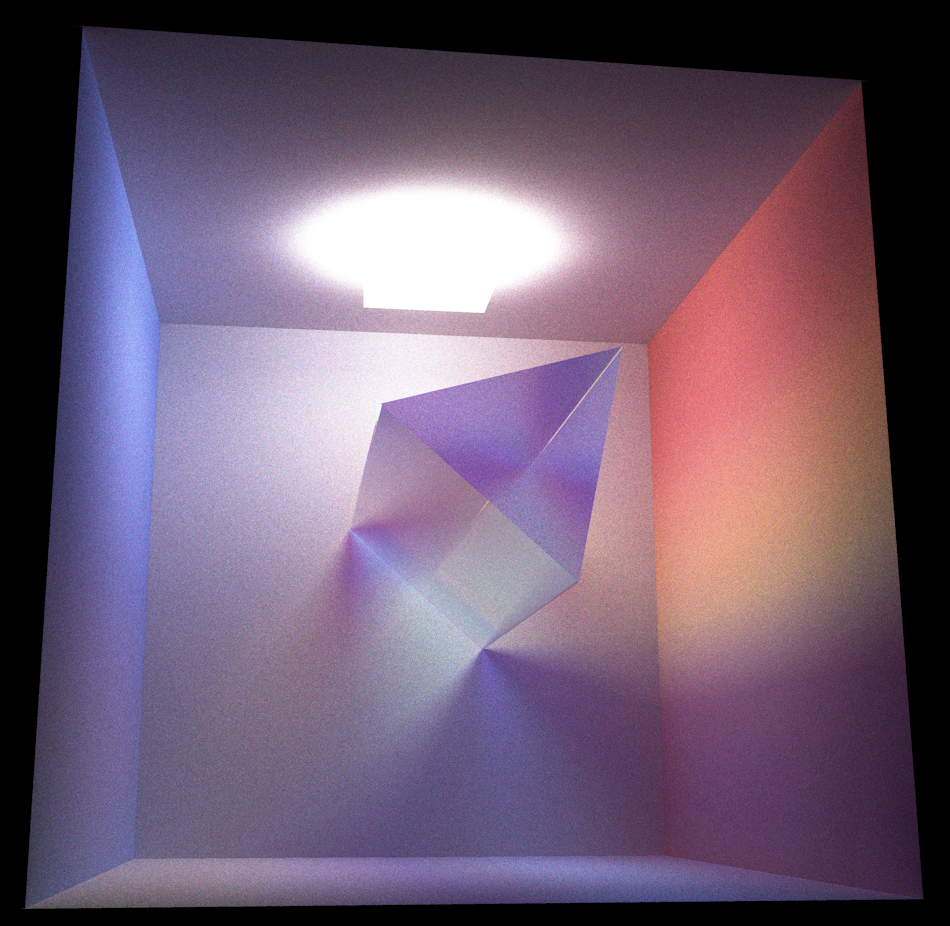
\includegraphics[width = 6 in]{fig7.png}
  \caption{ Note the refraction caustic, with 20-channel chromatic aberration.
}
\end{figure}


\begin{figure} 
\centering
  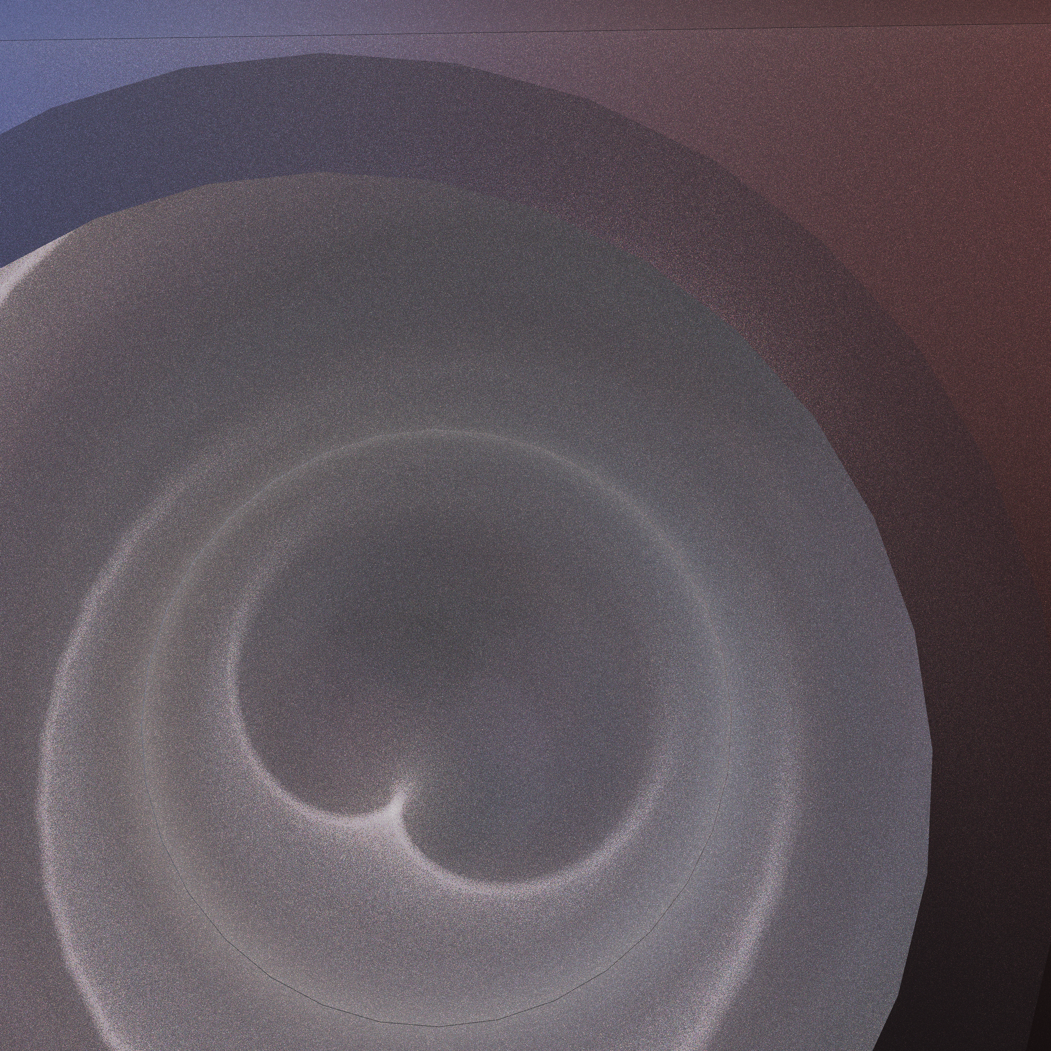
\includegraphics[width = 6 in]{fig8.png}
  \caption{ Note the nephroid reflection caustic at the bottom of a hollow cylinder.
}
\end{figure}


\begin{figure} 
\centering
  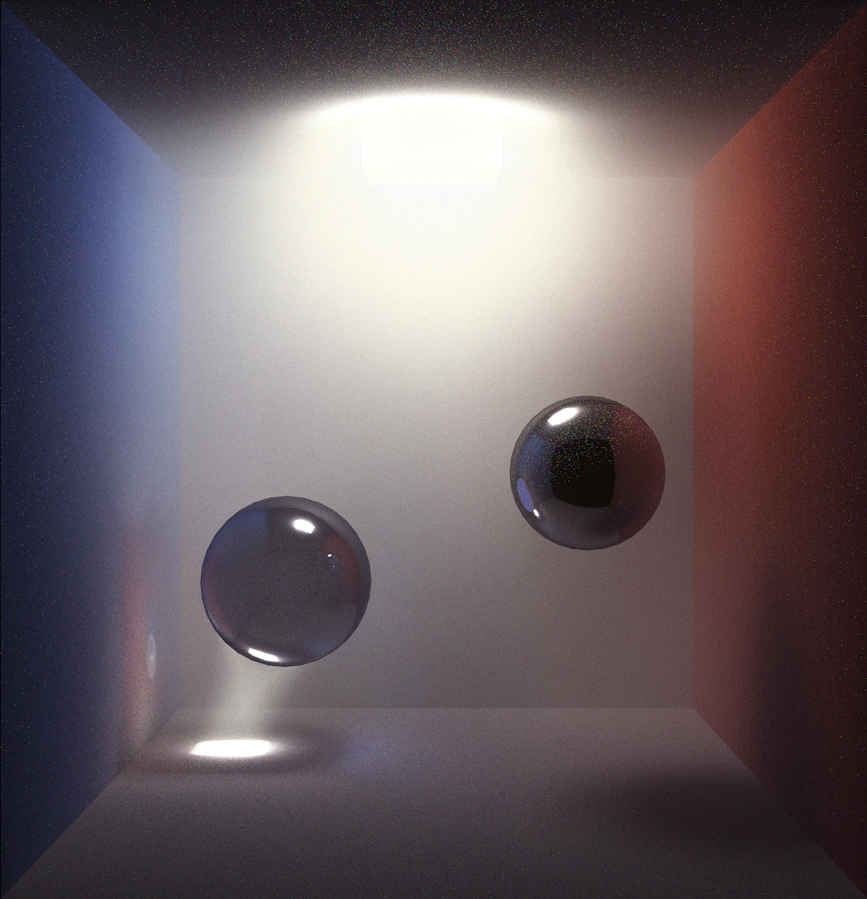
\includegraphics[width = 6 in]{fig9.png}
  \caption{ Note that the experimental fog lights up because of the caustic.
%These images are an homage to Canadian 3-D graphics companies from earlier days, such as Alias, ATI, Matrox, and Softimage.
}
\end{figure}


\begin{figure} 
\centering
  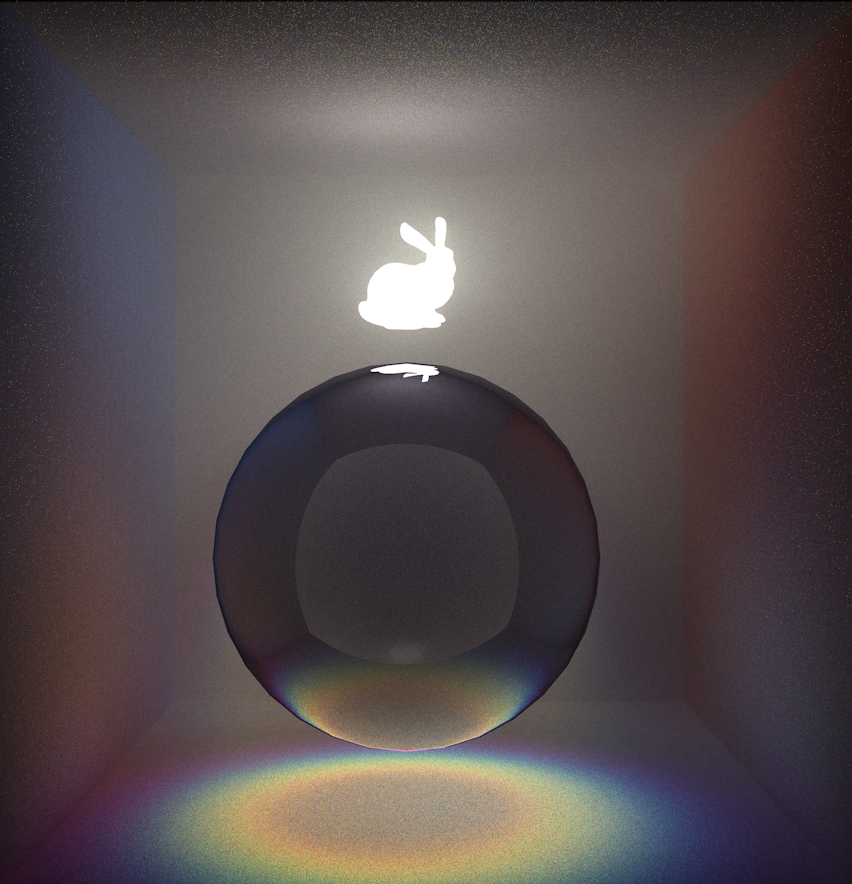
\includegraphics[width = 6 in]{fig10.png}
  \caption{ Stanford bunny light.
}
\end{figure}





\end{document}





